\documentclass[letterpaper]{article}

\usepackage{fancyhdr}
\usepackage{extramarks}
\usepackage{amsmath}
\usepackage{amsthm}
\usepackage{amsfonts}
\usepackage{tikz}
\usepackage[plain]{algorithm}
\usepackage{algpseudocode}
\usepackage{amsmath}
\usepackage{verbatim}
\usepackage{graphicx}
\usepackage{epstopdf}

\usetikzlibrary{automata,positioning}

%
% Basic Document Settings
%

\topmargin=-0.45in
\evensidemargin=0in
\oddsidemargin=0in
\textwidth=6.5in
\textheight=9.0in
\headsep=0.25in

\linespread{1.1}

\pagestyle{fancy}
\lhead{\hmwkAuthorName}
%\chead{\hmwkClass\ (\hmwkClassInstructor): \hmwkTitle}
\rhead{\hmwkAuthorUNI}
\lfoot{\lastxmark}
\cfoot{\thepage}

\renewcommand\headrulewidth{0.4pt}
\renewcommand\footrulewidth{0.4pt}

\setlength\parindent{0pt}

%
% Create Problem Sections
%

\newcommand{\enterProblemHeader}[1]{
    %\nobreak\extramarks{}{Problem \arabic{#1} continued on next page\ldots}\nobreak{}
    %\nobreak\extramarks{Problem \arabic{#1} (continued)}{Problem \arabic{#1} continued on next page\ldots}\nobreak{}
}

\newcommand{\exitProblemHeader}[1]{
    %\nobreak\extramarks{Problem \arabic{#1} (continued)}{Problem \arabic{#1} continued on next page\ldots}\nobreak{}
    \stepcounter{#1}
    %\nobreak\extramarks{Problem \arabic{#1}}{}\nobreak{}
}

\setcounter{secnumdepth}{0}
\newcounter{partCounter}
\newcounter{homeworkProblemCounter}
\setcounter{homeworkProblemCounter}{1}
\nobreak\extramarks{Problem \arabic{homeworkProblemCounter}}{}\nobreak{}

\newenvironment{homeworkProblem}{
    \section{Problem \arabic{homeworkProblemCounter}}
    \setcounter{partCounter}{0}
    \enterProblemHeader{homeworkProblemCounter}
}{
    \exitProblemHeader{homeworkProblemCounter}
}

%
% Homework Details
%   - Title
%   - Due date
%   - Class
%   - Section/Time
%   - Instructor
%   - Author
%

\newcommand{\hmwkTitle}{Homework\ \#1}
\newcommand{\hmwkDueDate}{September 19, 2017}
\newcommand{\hmwkClass}{PROBABILITY}
%\newcommand{\hmwkClassTime}{Section 005}
\newcommand{\hmwkClassInstructor}{Professor Regina}
\newcommand{\hmwkAuthorName}{Fan Yang}
\newcommand{\hmwkAuthorUNI}{UNI: fy2232}

%
% Title Page
%

\title{
    \vspace{2in}
    \textmd{\textbf{\hmwkClass:\ \hmwkTitle}}\\
    \normalsize\vspace{0.1in}\small{Due\ on\ \hmwkDueDate}\\
    \vspace{0.1in}\large{\textit{\hmwkClassInstructor}}
    \vspace{3in}
}

\author{\textbf{\hmwkAuthorName}\\
    \text{\hmwkAuthorUNI}}
\date{}

\renewcommand{\part}[1]{\textbf{\large Part \Alph{partCounter}}\stepcounter{partCounter}\\}

%
% Various Helper Commands
%

% Useful for algorithms
\newcommand{\alg}[1]{\textsc{\bfseries \footnotesize #1}}

% For derivatives
\newcommand{\deriv}[1]{\frac{\mathrm{d}}{\mathrm{d}x} (#1)}

% For partial derivatives
\newcommand{\pderiv}[2]{\frac{\partial}{\partial #1} (#2)}

% Integral dx
\newcommand{\dx}{\mathrm{d}x}

% Alias for the Solution section header
\newcommand{\solution}{\textbf{\large Solution}}

% Probability commands: Expectation, Variance, Covariance, Bias
\newcommand{\E}{\mathrm{E}}
\newcommand{\Var}{\mathrm{Var}}
\newcommand{\Cov}{\mathrm{Cov}}
\newcommand{\Bias}{\mathrm{Bias}}

\begin{document}

\maketitle
\setcounter{page}{0}
\thispagestyle{empty}

\pagebreak

\begin{homeworkProblem}     %1

    \textbf{(a)}
    denote H for heads and T for tails.
    \[
        \begin{split}
            S=
                    \{&(H,H,H),(H,H,T),(H,T,H),(H,T,T)
            \\
            &(T,H,H),(T,H,T),(T,T,H),(T,T,T) \}
            \\
        \end{split}
    \]

    \textbf{(b)}

    \[
        \begin{split}
            & A=\{(H,H,T),(H,T,H),(T,H,H),(H,H,H)\}
            \\
            &B= \{(H,H,T),(H,H,H)\}
            \\
            &C=\{(H,H,T),(H,T,T),(T,H,T),(T,T,T)\}
        \end{split}
    \]
    \textbf{(c)}

    \[
        \begin{split}
            1)&~A^c=\{(H,T,T),(T,H,T),(T,T,H),(T,T,T)\}
            \\
            2)&~A \cap B = \{(H,H,T),(H,H,H)\}=B
            \\
            3)&~A \cup C = \{ (H,H,T),(H,T,H),(T,H,H),(H,H,H),(H,T,T),(T,H,T),(T,T,T)\}
        \end{split}
    \]

\end{homeworkProblem}

\begin{homeworkProblem}%2

    \textbf{(a)}
    denote H for heads and T for tails.
    \[
        \begin{split}
            &\text{number of sample space is } \left( \begin{array}{c}52\\5\end{array} \right)
            \\
            &\text{number of choices of  suits is }\left(\begin{array}{c}4\\1\end{array}\right)
            \\
            &P=\frac{ \# of suits}{\# of sample~space}\\
            &=\frac{\left(\begin{array}{c}4\\1\end{array}\right)}{\left( \begin{array}{c}52\\5\end{array} \right)}\\
            &=\frac{1}{649740}
            \\
        \end{split}
    \]

    \textbf{(b)}

    \[
        \begin{split}
            &\text{list possible situations as (A2345)...(10JQKA),we know there are 10 choices of value and}\\
            &\text{4 choices of suit. But we should exclude Royal Flush}\\
            \\
            &P= \frac{10*4-4}{\left( \begin{array}{c}52\\5\end{array} \right)}\\
            &~~\approx 1.39\times 10^{-5}\\
        \end{split}
    \]
    \textbf{(c)}

    \[
        \begin{split}
            &\text{there are 13 choices of value}\\
            &\text{as for the other card, there are 48 choices}
            \\
            &P= \frac{13*48}{\left( \begin{array}{c}52\\5\end{array} \right)}\\
            &~~=\frac{1}{4165}
        \end{split}
    \]
    \textbf{(d)}

    \[
        \begin{split}
            &\text{since the 5 cards have same suits, they should not have same value}\\
            &\text{there are }\left( \begin{array}{c}13\\5\end{array} \right)\text{ choices of value}\\
            &\text{there are 4 choices of suit}\\
            &\text{What's more, we should exclude Royal Flush and Straight Flush}
            \\
            &P= \frac{\left( \begin{array}{c}13\\5\end{array} \right)*4-4-36}{\left( \begin{array}{c}52\\5\end{array} \right)}\\
            &~~=\frac{1277}{649740}\approx1.97\times 10^{-3}\\
        \end{split}
    \]

    \textbf{(e)}

    \[
        \begin{split}
            &\text{Choose 3 same cards first:There are 13 choices of value and $\left( \begin{array}{c}4\\3\end{array} \right)$ choices of suit}\\
            &\text{As for the other two cards:There are $\left( \begin{array}{c}52-4\\2\end{array} \right)$ choices}\\
            &P= \frac{13*4*\left( \begin{array}{c}52-4\\2\end{array} \right)}{\left( \begin{array}{c}52\\5\end{array} \right)}\\
            &~~=\frac{94}{4165}
        \end{split}
    \]
    \textbf{(f)}

    \[
        \begin{split}
            &\text{there are $\left(\begin{array}{c}13\\2\end{array} \right)$ choices of value.}\\
            &\text{there are $\left(\begin{array}{c}4\\2\end{array} \right)*\left(\begin{array}{c}4\\2\end{array} \right)$ choices of value.}\\
            &\text{as for the last cards, there are only 52-4-4 choices.}\\
            &P= \frac{\left(\begin{array}{c}13\\2\end{array} \right)*\left(\begin{array}{c}4\\2\end{array} \right)*\left(\begin{array}{c}4\\2\end{array} \right)*(52-4-4)}{\left( \begin{array}{c}52\\5\end{array} \right)}\\
            &~~=\frac{198}{4165}
        \end{split}
    \]

\end{homeworkProblem}

\begin{homeworkProblem}     %3

    \textbf{(a)}
    \[
        \begin{split}
    &\text{there are 16 choices for women president. And there are 48 choices for president}\\
    &so~Pr(E)=\frac{16}{48}=\frac{1}{3}\\
        &\text{there are 32 choices for men vice president.
        And there are 48 choices for vice president}\\
        &so~Pr(F)=\frac{32}{48}
        ~=\frac{2}{3}\\
        &\text{there are}16*15+32*31\text{ choices for president of same sex}\\
        &\text{there are 48*47 choices for president}\\
        &so~Pr(G)=\frac{16*15+32*31}{48*47}\\
        &=\frac{77}{141}\\
        \end{split}
    \]

    \textbf{(b)}

    \[
        \begin{split}
            & E\cap F \text{ represent president is woman and vice president is man}\\
            &\text{there are 16*32 choices for this situation}\\
            & E\cup F \text{ represent president is woman or vice president is man}\\
            &\text{there are 16*32+16*15+32*31 choices for this situation}\\
            & E\cap F\cap G \text{ does not make sense}\\
            &\text{there are 0 choices for this situation}\\
            &Pr(E\cap F)= \frac{16*32}{48*47}=\frac{32}{141}\\
            &Pr(E\cup F)= \frac{16*32+16*15+32*31}{48*47}=\frac{109}{141}\\
            &Pr(E\cap F\cap G)=0
        \end{split}
    \]
    \textbf{(c)}

    \[
        \begin{split}
        &Pr(G|E\cup F)=\frac{Pr(G\cap (E\cup F))}{Pr(E\cup F)}\\
        &G\cap (E\cup F)\text{represent two president are of same sex}=G\\
        &therefore~Pr(G|E\cup F)=\frac{Pr(G)}{Pr(E\cup F)}
        =\frac{\frac{77}{141}}{\frac{109}{141}}=\frac{77}{109}\\
        \end{split}
    \]

\end{homeworkProblem}

\begin{homeworkProblem}     %4
    \[
        \begin{split}
    &\text{consider the event as inserting four adjacent aces into 48 shuffled cards}\\
    &\text{\# of order of adjacent aces are 4*3*2*1}\\
    &\text{\# of choices of inserting the four adjacent are 49!} \\
    &\text{\# in sample space is 52!}\\
    &therefore~P=\frac{4*3*2*49!}{52!}\approx 1.81\times 10^{-4}\\
        \end{split}
    \]
\end{homeworkProblem}

\begin{homeworkProblem}

    \textbf{(a)}
    \[
        \begin{split}
    &\text{\# of the sample space}=
        \left(\begin{array}{c}60\\30\end{array}\right)\\
        &\text{there are} 2\times\left(\begin{array}{c}60-5\\30\end{array}\right) \text{choices for this situation.}\\
        &so~P=\frac{2\times\left(\begin{array}{c}55\\30\end{array}\right)}
        {\left(\begin{array}{c}60\\30\end{array}\right)}\\
        &=\frac{117}{2242}\\
        \end{split}
    \]

    \textbf{(b)}

    \[
        \begin{split}
            &\text{\# of the sample space}=
        \left(\begin{array}{c}60\\30\end{array}\right)\\
        &\text{there are} 2*\left(\begin{array}{c}5\\4\end{array}\right)*
         \left(\begin{array}{c}60-5\\30-4\end{array}\right)
         \text{choices for this situation.}\\
        &so~P=\frac{2\times\left(\begin{array}{c}5\\4\end{array}\right)*
        \left(\begin{array}{c}60-5\\30-4\end{array}\right)}
        {\left(\begin{array}{c}60\\30\end{array}\right)}\\
        &=\frac{675}{2242}\\
        \end{split}
    \]

    \textbf{(c)}

    \[
        \begin{split}
            &\text{\# of the sample space}=
        \left(\begin{array}{c}60\\30\end{array}\right)\\
        &\text{there are} 2\times\left(\begin{array}{c}60-5\\30-1\end{array}\right)
         \text{choices for this situation.}\\
        &so~P=\frac{2\times\left(\begin{array}{c}60-5\\30-1\end{array}\right)}
        {\left(\begin{array}{c}60\\30\end{array}\right)}\\
        &=\frac{135}{2242}\\
        \end{split}
    \]

\end{homeworkProblem}

\begin{homeworkProblem}     %6

    \textbf{(a)}
    \[
        \begin{split}
        &\text{this event could be either first up then down or first down then up}\\
        &so~P=p*(1-p)+(1-p)*p\\
        &=2p(1-p)
        \end{split}
    \]

    \textbf{(b)}

    \[
        \begin{split}
        &\text{there should be 1 day down and 2 days up}\\
        &so~P=\left(\begin{array}{c}3\\1\end{array}\right)*
        p^2 *(1-p)\\
        &=3p^2 (1-p)\\
        \end{split}
    \]

    \textbf{(c)}

    \[
        \begin{split}
        & \text{denote E for price increasing on the first day,then}~Pr(E)=p\\
        & \text{denote F for after three days price increased by 1,then}~Pr(F)=3p^2 (1-p)\\
        & \text{the probability that the first day price goes up and three days later price still increased by 1 should be}\\
        &Pr(E\cap F)=p*\left(\begin{array}{c}2\\1\end{array}\right)*p*(1-p)\\
        &=2p^2 (1-p)\\
        &Pr(E|F)=\frac{Pr(E\cap F)}{Pr(F)}\\
        &=\frac{2p^2 (1-p)}{3p^2 (1-p)}\\
        &=\frac{2}{3}\\
        \end{split}
    \]

\end{homeworkProblem}


\begin{homeworkProblem}     %7
    \[
        \begin{split}
        &\text{under strategy (a),the answer could be correct when either husband or wife gives the correct answer.}\\
        &so~P=\frac{1}{2}*p+\frac{1}{2}*p=p\\
        &\text{under strategy (b),the answer could be correct in the following situations:.}\\
        &\text{1)husband correct wife correct and either of their answer to be given.} \\
        &\text{2)husband correct wife wrong and husband's answer is given.} \\
        &\text{3)wife correct husband wrong and wife's answer is given.}\\
        &so~P=p*p+\frac{1}{2}*p*(1-p)+\frac{1}{2}*p*(1-p)
        =p\\
        &\text{therefore,the two strategies have same efficiency.}\\
        \end{split}
    \]

\end{homeworkProblem}

\begin{homeworkProblem}     %8

    \textbf{(1)}
    \[
        \begin{split}
        &Pr(agree)=p*p+(1-p)*(1-p)=2p^2-2p+1\\
        &\text{from problem 7 we know }Pr(correct)=p\\
        &Pr(correct|agree)=\frac{Pr(correct\cap agree)}{Pr(agree)}
        =\frac{p*p}{2p^2-2p+1}=\frac{9}{13}\\
        \end{split}
    \]

    \textbf{(2)}
    \[
        \begin{split}
        &Pr(disagree)=p*(1-p)+(1-p)*p=2p(1-p)\\
        &Pr(correct\cap disagree)=\frac{1}{2}*p*(1-p)+\frac{1}{2}(1-p)*p=p(1-p)\\
        &Pr(correct|disagree)=\frac{Pr(correct\cap disagree)}{Pr(disagree)}
        =\frac{p(1-p)}{2p(1-p)}=\frac{1}{2}\\
        \end{split}
    \]

\end{homeworkProblem}

\begin{homeworkProblem}     %9
    \[
        \begin{split}
        &\text{we will calculate the chance that there is no head}\\
        &Pr_{(no~head)}=(1-p)^n.\\
        &\text{in contrast, the probability that at least one head is}\\
        &Pr_{(at~least~one~head)}=1-(1-p)^n\\
        &1-(1-p)^n\geq 0.5\Leftrightarrow (1-p)^n\leq 0.5\\
        &1-p\in [0,1];~so~n*log(1-p)\leq log(0.5)\\
        &\Leftrightarrow n\geq \frac{log(\frac{1}{2})}{log(1-p)}\\
        &\text{and p could not equal to 1}\\
        \end{split}
    \]

\end{homeworkProblem}

\begin{homeworkProblem}     %10
    \[
        \begin{split}
        &\text{denote the event a silver coin is found as E}\\
        &Pr(E)=\frac{1}{3}*\frac{1}{2}+\frac{1}{3}*1=\frac{1}{2}\\
        &\text{denote the event two silver coins is found as F}\\
        &Pr(F)=\frac{1}{3}\\
        &Pr(F|E)=\frac{Pr(F\cap E)}{Pr(E)}\\
        &=\frac{Pr(F)}{Pr(E)}=\frac{\frac{1}{3}}{\frac{1}{2}}=\frac{2}{3}\\
        \end{split}
    \]

\end{homeworkProblem}

\begin{homeworkProblem}     %11

    \textbf{(a)}
    \[
        \begin{split}
        &\text{let's separate this event into two parts:}\\
        &\text{a)a red ball is drawn from A; b)any ball other than red is drawn form A}\\
        &then~P=\frac{4}{4+3+2}*\frac{3}{3+3+4}
        +\frac{3+2}{4+3+2}*\frac{2}{2+3+4+1}
        =\frac{11}{45}\\
        \end{split}
    \]

    \textbf{(b)}

    \[
        \begin{split}
        &\text{denote E as drawn red from A and F as drawn red from B}\\
        &\text{from part (a) we get}~ Pr(F)=\frac{11}{45}\\
        &Pr(E\cap F)=\frac{4}{4+3+2}*\frac{3}{3+3+4}=\frac{2}{15}\\
        &Pr(E|F)=\frac{Pr(E\cap F)}{Pr(F)}\\
        &=\frac{Pr(E\cap F)}{Pr(F)}=\frac{\frac{2}{15}}{\frac{11}{45}}
        =\frac{6}{11}\\
        \end{split}
    \]

\end{homeworkProblem}

\begin{homeworkProblem}     %12 #7 on page 21

    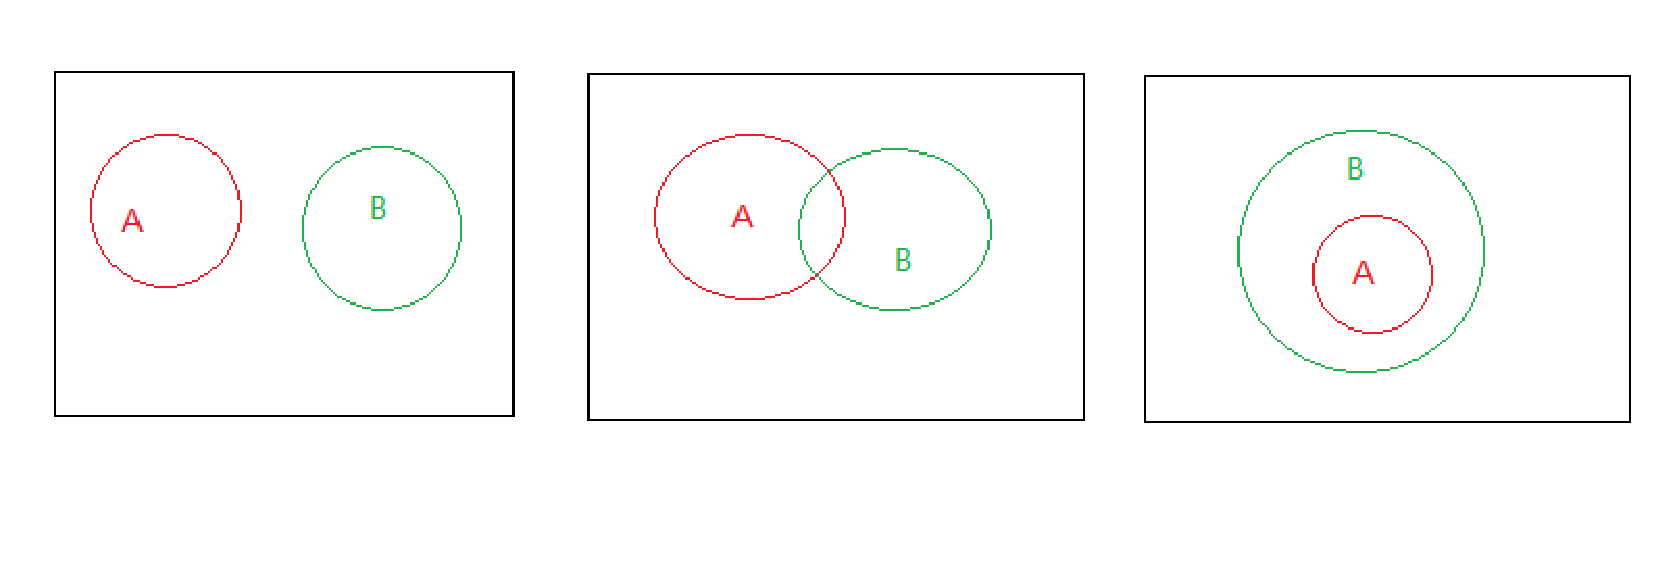
\includegraphics[height=2in]{prob_hw1_pic1}

    \[
        \begin{split}
        &\text{from the above venn diagram,we come to the following conclusion:}\\
        &\text{As for the right diagram, there is no intersection between A and B, but Pr(A)+Pr(B)=1.1$>$1, so}\\
        &\text{there should be intersection}\\
        &\text{1) when A and B have the smallest intersection, }~Pr(A\cup B)=1\\
        &Pr(A\cap B)=Pr(A)+Pr(B)-Pr(A\cup B)=0.1\\
        &\text{2) when B is a sub set of A, then}~Pr(A\cap B)~\text{get the maximum value 0.4.}\\
        \end{split}
    \]

\end{homeworkProblem}

\begin{homeworkProblem}     %13    #3 on page 25.

    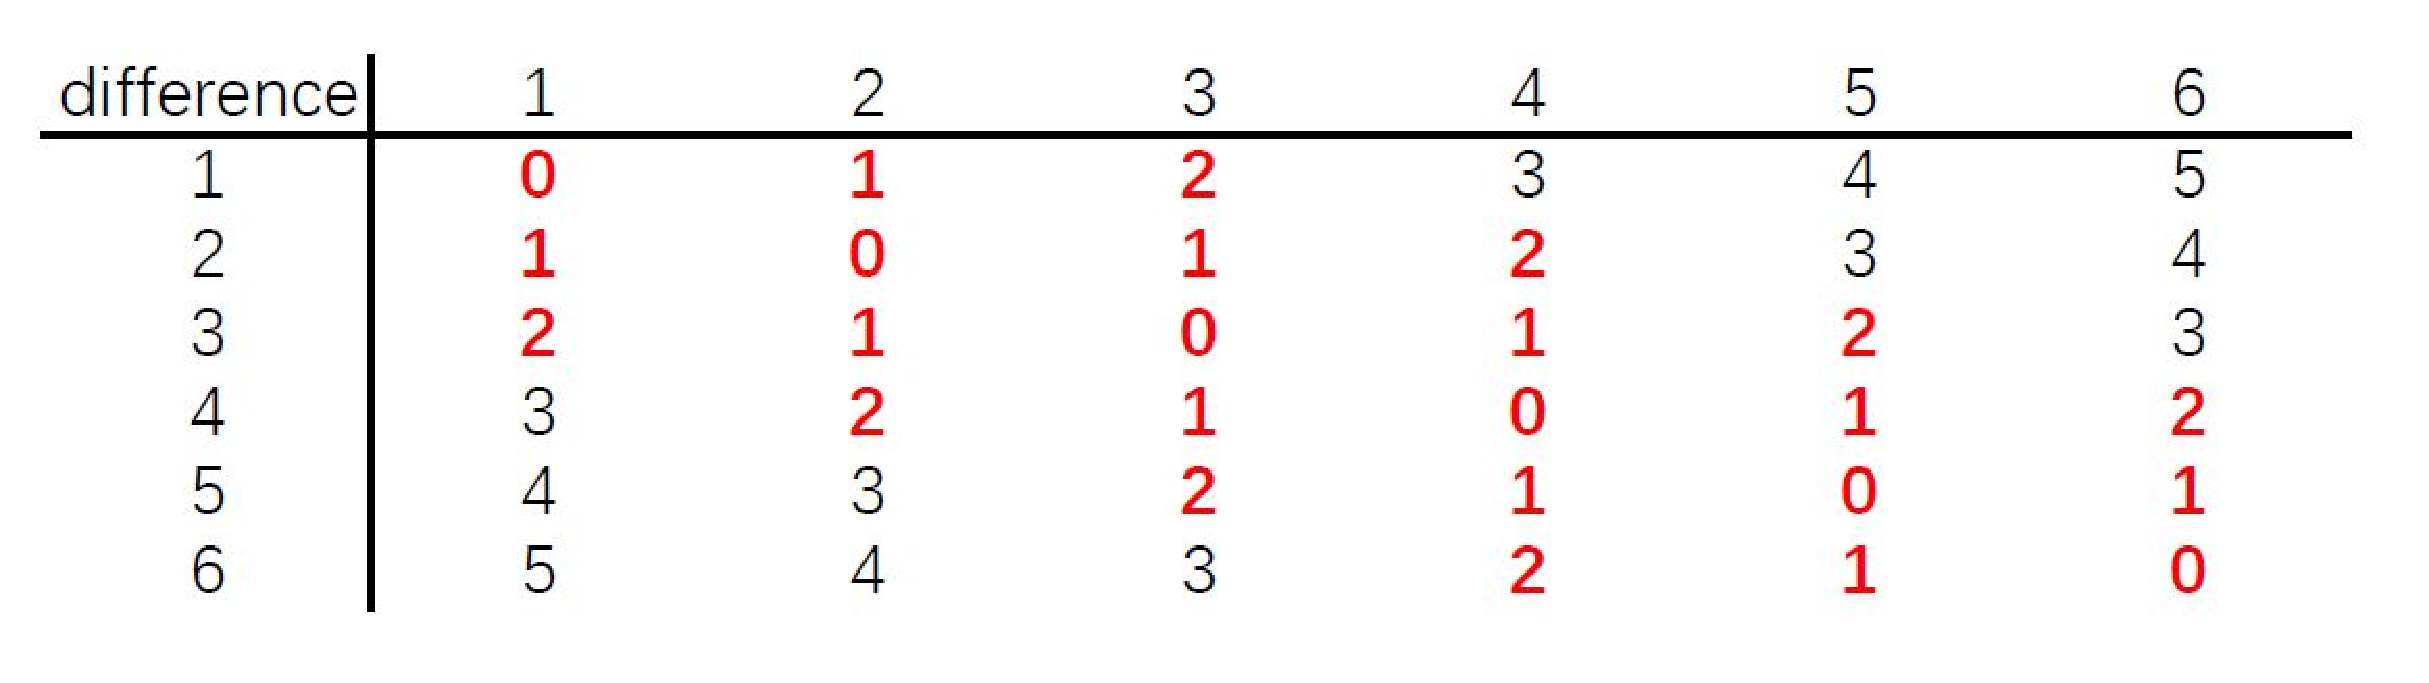
\includegraphics[height=1.5in]{prob_hw1_pic2}

    \[
        \begin{split}
        &\text{as the graph above depicts, we get:}\\
        &P=\frac{24}{36}=\frac{2}{3}\\
        \end{split}
    \]

\end{homeworkProblem}

\begin{homeworkProblem}     %14    #7 on page 32.
    \[
        \begin{split}
        &\text{the number in sample space should be}20^12\\
        &\text{the situation that no box have more than one ball is the same as there are}\\
        &\text{ 12 boxes with one box each only and 8 empty boxes,but order matters.}\\
        &\text{so number of choices of this situation is }
        \begin{array}{c}20!\\12!\end{array}\\
        &therefore~P=\frac{\left(\begin{array}{c}20!\\12!\end{array}\right)}{20^12}\\
        &=1.24\times10^{-6}\\
        \end{split}
    \]

\end{homeworkProblem}

\begin{homeworkProblem}     %15    #12 on page 41
    \[
        \begin{split}
        &\text{the number in sample space should be}
        \left(\begin{array}{c}35\\10 \end{array} \right)\\
        &\text{number of choices of this situation is }
        \left(\begin{array}{c}35-2\\10-2\end{array}\right)+
        \left(\begin{array}{c}35-2\\10\end{array}\right)\\
        &=\left(\begin{array}{c}33\\8\end{array}\right)+
        \left(\begin{array}{c}33\\10\end{array}\right)\\
        &so~P=\frac{\left(\begin{array}{c}33\\8\end{array}\right)+
        \left(\begin{array}{c}33\\10\end{array}\right)}{\left(\begin{array}{c}35\\10 \end{array} \right)}\\
        &=\frac{69}{119}\\
        \end{split}
    \]

\end{homeworkProblem}

\begin{homeworkProblem}     %16    #8 on page 46.
    \[
        \begin{split}
        &\text{the number in sample space should be}
        \left(\begin{array}{c}52\\13,13,13,13 \end{array} \right)\\
        &\text{number of choices of this situation is }
        \left(\begin{array}{c}12\\3,3,3,3\end{array}\right)*
        \left(\begin{array}{c}40\\10,10,10,10\end{array}\right)\\
        &so~P=\frac{\left(\begin{array}{c}12\\3,3,3,3\end{array}\right)*
        \left(\begin{array}{c}40\\10,10,10,10\end{array}\right)}
        {\left(\begin{array}{c}52\\13,13,13,13 \end{array} \right)}\\
        &=\frac{\frac{12!}{(3!)^4}*\frac{40!}{(10!)^4}}{\frac{52!}{(13!)^4}}\\
        &=\frac{\frac{12!}{(3!)^4}*\frac{40!}{(10!)^4}}{\frac{52!}{(13!)^4}}\\
        &=\frac{148933}{4594023}\approx 0.0324
        \end{split}
    \]

\end{homeworkProblem}

\begin{homeworkProblem}     %17    #6 on page 50.
    \[
        \begin{split}
        &\text{the number in sample space should be}
        \left(\begin{array}{c}30*3\\10 \end{array} \right)\\
        &\text{number of choices of missing one color is }
        3\times\left(\begin{array}{c}30*3\times2\\10\end{array}\right)-2*
        \left(\begin{array}{c}30\\10\end{array}\right)\\
        &\text{number of choices of missing two color is }
        3*\left(\begin{array}{c}30\\10\end{array}\right)\\
        &so~P=\frac{\left(\begin{array}{c}30*2\\10\end{array}\right)-2*
        \left(\begin{array}{c}30\\10\end{array}\right)
        +3*\left(\begin{array}{c}30\\10\end{array}\right)}
        {\left(\begin{array}{c}30*3\\10 \end{array} \right)}\\
        &=\frac{2357}{59590}\approx 0.040
        \end{split}
    \]

\end{homeworkProblem}

\end{document}
